% Foliensatz: "AFu-Kurs nach DJ4UF" von DK0TU, Amateurfunkgruppe der TU Berlin
% Lizenz: CC BY-NC-SA 3.0 de (http://creativecommons.org/licenses/by-nc-sa/3.0/de/)
% Autoren: Martin Deutschmann <martin.deutschmann@campus.tu-berlin.de>
% Korrekturen: Lars Weiler <dc4lw@darc.de>, Sebastian Lange <dl7bst@dk0tu.de>

\documentclass[aspectratio=169]{beamer}

\usepackage[ngerman]{babel} % deutsche Worttrennung etc.
\usepackage[utf8]{inputenc} % UTF8 Text

\usepackage[super, comma, numbers, square, sort]{natbib}

\usepackage{hyperref}       % Hyperref Package für bessere Referenzen (todo)
\hypersetup{
	colorlinks=false,       %   false: boxed links; true: colored links
    %linkcolor=white,       %   color of internal links (change box color with linkbordercolor)
    citecolor=red,          %   color of links to bibliography
    filecolor=white,        %   color of file links
    urlcolor=blue           %   color of external links
}

\usepackage{multirow}
\usepackage{wasysym}  % Math Symbols like \permil
%\usepackage{colortbl}
%\usepackage{subscript}
%\usepackage{caption}
%\usepackage{setspace}
%\usepackage{xcolor}        % benutze CodeListe

% Footnote
%\usepackage{hanging}
%
%\setbeamertemplate{footnote}{%
%  \hangpara{2em}{1}%
%  \makebox[2em][l]{\insertfootnotemark}\footnotesize\insertfootnotetext\par%
%}


%\usepackage{pgf}
%\usepackage{tikz}
%\usetikzlibrary{arrows,automata}
%\usetikzlibrary{positioning}
%
%\tikzset{
%    state/.style={
%           rectangle,
%           rounded corners,
%           draw=black, very thick,
%           minimum height=2em,
%           minimum width=2pt,
%           inner sep=2pt,
%           text centered,
%           },
%}

%\usepackage{listings}
%\lstset{basicstyle=\small, numberstyle=\tiny, extendedchars=true, numbers=left, numbersep=5pt}
%\lstset{showtabs=false, showspaces=false, showstringspaces=false}
%%\lstset{backgroundcolor=\color{white!75!lightgray}, , frame=single}
%%\lstset{backgroundcolor=\color{white}}
%%\lstset{backgroundcolor=none}
%\lstset{keywordstyle=\color{blue!50!gray},  identifierstyle=\color{black}}
%\lstset{commentstyle=\color{green!50!gray}, stringstyle=\color{red!50!gray}}
%\lstset{language=C, fontadjust=true, tabsize=2, breaklines=true}
%\lstset{backgroundcolor=\color{white!75!lightgray}, caption=\lstname, frame=single}
%\lstset{emphstyle=\color{black}\fbox}
%
%% Keine "Listing:"-Caption
%\captionsetup{labelformat=empty,labelsep=none}
%
%% für mathematische Umgebungen
%\usepackage{amsmath,amsfonts,amssymb}
%
%\lstdefinestyle{Bash}{
%language=Bash,
%frame=single,
%rulecolor=\color{black},
%backgroundcolor=\color{gray!50},
%keywordstyle=\color{black},
%identifierstyle=,
%commentstyle=\color{black},
%stringstyle=\color{magenta!65!white},
%showstringspaces=false,
%basicstyle=\footnotesize\ttfamily\color{black},
%numbers=none,
%breaklines=true,
%captionpos=b
%}

%\usepackage{listings}
%
%\lstdefinestyle{basic}{
%    captionpos=t,%
%    basicstyle=\footnotesize\ttfamily,%
%    numberstyle=\tiny,%
%    numbers=left,%
%    stepnumber=1,%
%    frame=single,%
%    showspaces=false,%
%    showstringspaces=false,%
%    showtabs=false,%
%    %
%    keywordstyle=\color{blue},%
%    identifierstyle=,%
%    commentstyle=\color{gray},%
%    stringstyle=\color{magenta}%
%}



% fließende Boxen haben keinen Abstand
%\fboxsep0mm

% inkludiere Creative Commons Helper
%%%%%%%%%%%%%%%%%%%%%%%%%%%%%%%%%%%%%%%%%%%%%%%%%%%%%%%%%%%%%%%%
%% ccBeamer 0.1, 2007-07-02                                   %%
%% Written by Sebastian Pipping <webmaster@hartwork.org>      %%
%% ---------------------------------------------------------- %%
%% Licensed under Creative Commons Attribution-ShareAlike 3.0 %%
%% http://creativecommons.org/licenses/by-sa/3.0/             %%
%%%%%%%%%%%%%%%%%%%%%%%%%%%%%%%%%%%%%%%%%%%%%%%%%%%%%%%%%%%%%%%%


%% Images
\newcommand{\CcImageBy}[1]{%
	
\includegraphics[scale=#1]{texdata/creative_commons/cc_by_30.pdf}%
}
\newcommand{\CcImageCc}[1]{%
	
\includegraphics[scale=#1]{texdata/creative_commons/cc_cc_30.pdf}%
}
\newcommand{\CcImageDevNations}[1]{%
	
\includegraphics[scale=#1]{texdata/creative_commons/cc_dev_nations_30.pdf}%
}
\newcommand{\CcImageNc}[1]{%
	
\includegraphics[scale=#1]{texdata/creative_commons/cc_nc_30.pdf}%
}
\newcommand{\CcImageNd}[1]{%
	
\includegraphics[scale=#1]{texdata/creative_commons/cc_nd_30.pdf}%
}
\newcommand{\CcImagePd}[1]{%
	
\includegraphics[scale=#1]{texdata/creative_commons/cc_pd_30.pdf}%
}
\newcommand{\CcImageSa}[1]{%
	
\includegraphics[scale=#1]{texdata/creative_commons/cc_sa_30.pdf}%
}
\newcommand{\CcImageSampling}[1]{%
	
\includegraphics[scale=#1]{texdata/creative_commons/cc_sampling_30.pdf}%
}
\newcommand{\CcImageSamplingPlus}[1]{%
	
\includegraphics[scale=#1]{texdata/creative_commons/cc_sampling_plus_30.pdf}%
}


%% Groups
\newcommand{\CcGroupBy}[2]{% zoom, gap
	\CcImageCc{#1}\hspace*{#2}\CcImageBy{#1}%
}
\newcommand{\CcGroupByNc}[2]{% zoom, gap
	\CcImageCc{#1}\hspace*{#2}\CcImageBy{#1}\hspace*{#2}\CcImageNc{#1}%
}
\newcommand{\CcGroupByNcNd}[2]{% zoom, gap
	\CcImageCc{#1}\hspace*{#2}\CcImageBy{#1}\hspace*{#2}\CcImageNc{#1}\hspace*{#2}\CcImageNd{#1}%
}
\newcommand{\CcGroupByNcSa}[2]{% zoom, gap
	\CcImageCc{#1}\hspace*{#2}\CcImageBy{#1}\hspace*{#2}\CcImageNc{#1}\hspace*{#2}\CcImageSa{#1}%
}
\newcommand{\CcGroupByNd}[2]{% zoom, gap
	\CcImageCc{#1}\hspace*{#2}\CcImageBy{#1}\hspace*{#2}\CcImageNd{#1}%
}
\newcommand{\CcGroupBySa}[2]{% zoom, gap
	\CcImageCc{#1}\hspace*{#2}\CcImageBy{#1}\hspace*{#2}\CcImageSa{#1}%
}
\newcommand{\CcGroupDevNations}[2]{% zoom, gap
	\CcImageCc{#1}\hspace*{#2}\CcImageDevNations{#1}%
}
\newcommand{\CcGroupNcSampling}[2]{% zoom, gap
	\CcImageCc{#1}\hspace*{#2}\CcImageNc{#1}\hspace*{#2}\CcImageSampling{#1}%
}
\newcommand{\CcGroupPd}[1]{% zoom
	\CcImagePd{#1}%
}
\newcommand{\CcGroupSampling}[1]{% zoom
	\CcImageSampling{#1}%
}
\newcommand{\CcGroupSamplingPlus}[1]{% zoom
	\CcImageSamplingPlus{#1}%
}


%% Text
\newcommand{\CcLongnameBy}{Attribution}
\newcommand{\CcLongnameByNc}{Attribution-NonCommercial}
\newcommand{\CcLongnameByNcNd}{Attribution-NoDerivs}
\newcommand{\CcLongnameByNcSa}{Attribution-NonCommercial-ShareAlike}
\newcommand{\CcLongnameByNd}{Attribution-NoDerivs}
\newcommand{\CcLongnameBySa}{Attribution-ShareAlike}

\newcommand{\CcNote}[1]{% longname
	This work is licensed under the \textit{Creative Commons #1 3.0 License}.%
}


% generelles Thema auswählen
\usetheme{Goettingen} %Berlin spart ohne Sidebar allerdings angenehm Platz
% AnnArbor | Antibes | Bergen | Berkeley | Berlin | Boadilla | boxes | CambridgeUS | Copenhagen | Darmstadt | default | Dresden | Frankfurt | Goettingen | Hannover | Ilmenau | JuanLesPins | Luebeck | Madrid | Malmoe | Marburg | Montpellier | PaloAlto | Pittsburgh | Rochester | Singapore | Szeged | Warsaw

% Farben wählen
\usecolortheme{beetle}
% beaver | beetle | crane | default | dolphin | dove | fly | lily | orchid | rose | seagull | seahorse | sidebartab | structure | whale | wolverine

% Setze alle Farben auf Grau und Weiß
%\definecolor{craneorange}{RGB}{64,64,64}
%\definecolor{craneblue}{RGB}{255,255,255}

% Schriftart wählen
\usefonttheme{default}
% default | professionalfonts | serif | structurebold | structureitalicserif | structuresmallcapsserif

% Innere Themen(Kopf-, Fuß-, Sidebar usw)
%\useinnertheme{default}
\useinnertheme{circles}
% default | inmargin | rectangles | rounded | circles

% Äußere Themen (Anordnung der inneren, grenzen der Folien etc.)
\useoutertheme{infolines}
% default | infolines | miniframes | shadow | sidebar | smoothbars | smoothtree | split | tree

% Deaktiviere Navigations-Symbole ({} -> leer)
\setbeamertemplate{navigation symbols}{}
%\setbeamertemplate{navigation symbols}{\large \ifnum \insertframenumber <10 0\fi\insertframenumber/\inserttotalframenumber\vspace*{0.2ex}}

% Zeige ein Hintergrundbild
\setbeamertemplate{background canvas}{
        \hspace*{-2.0cm}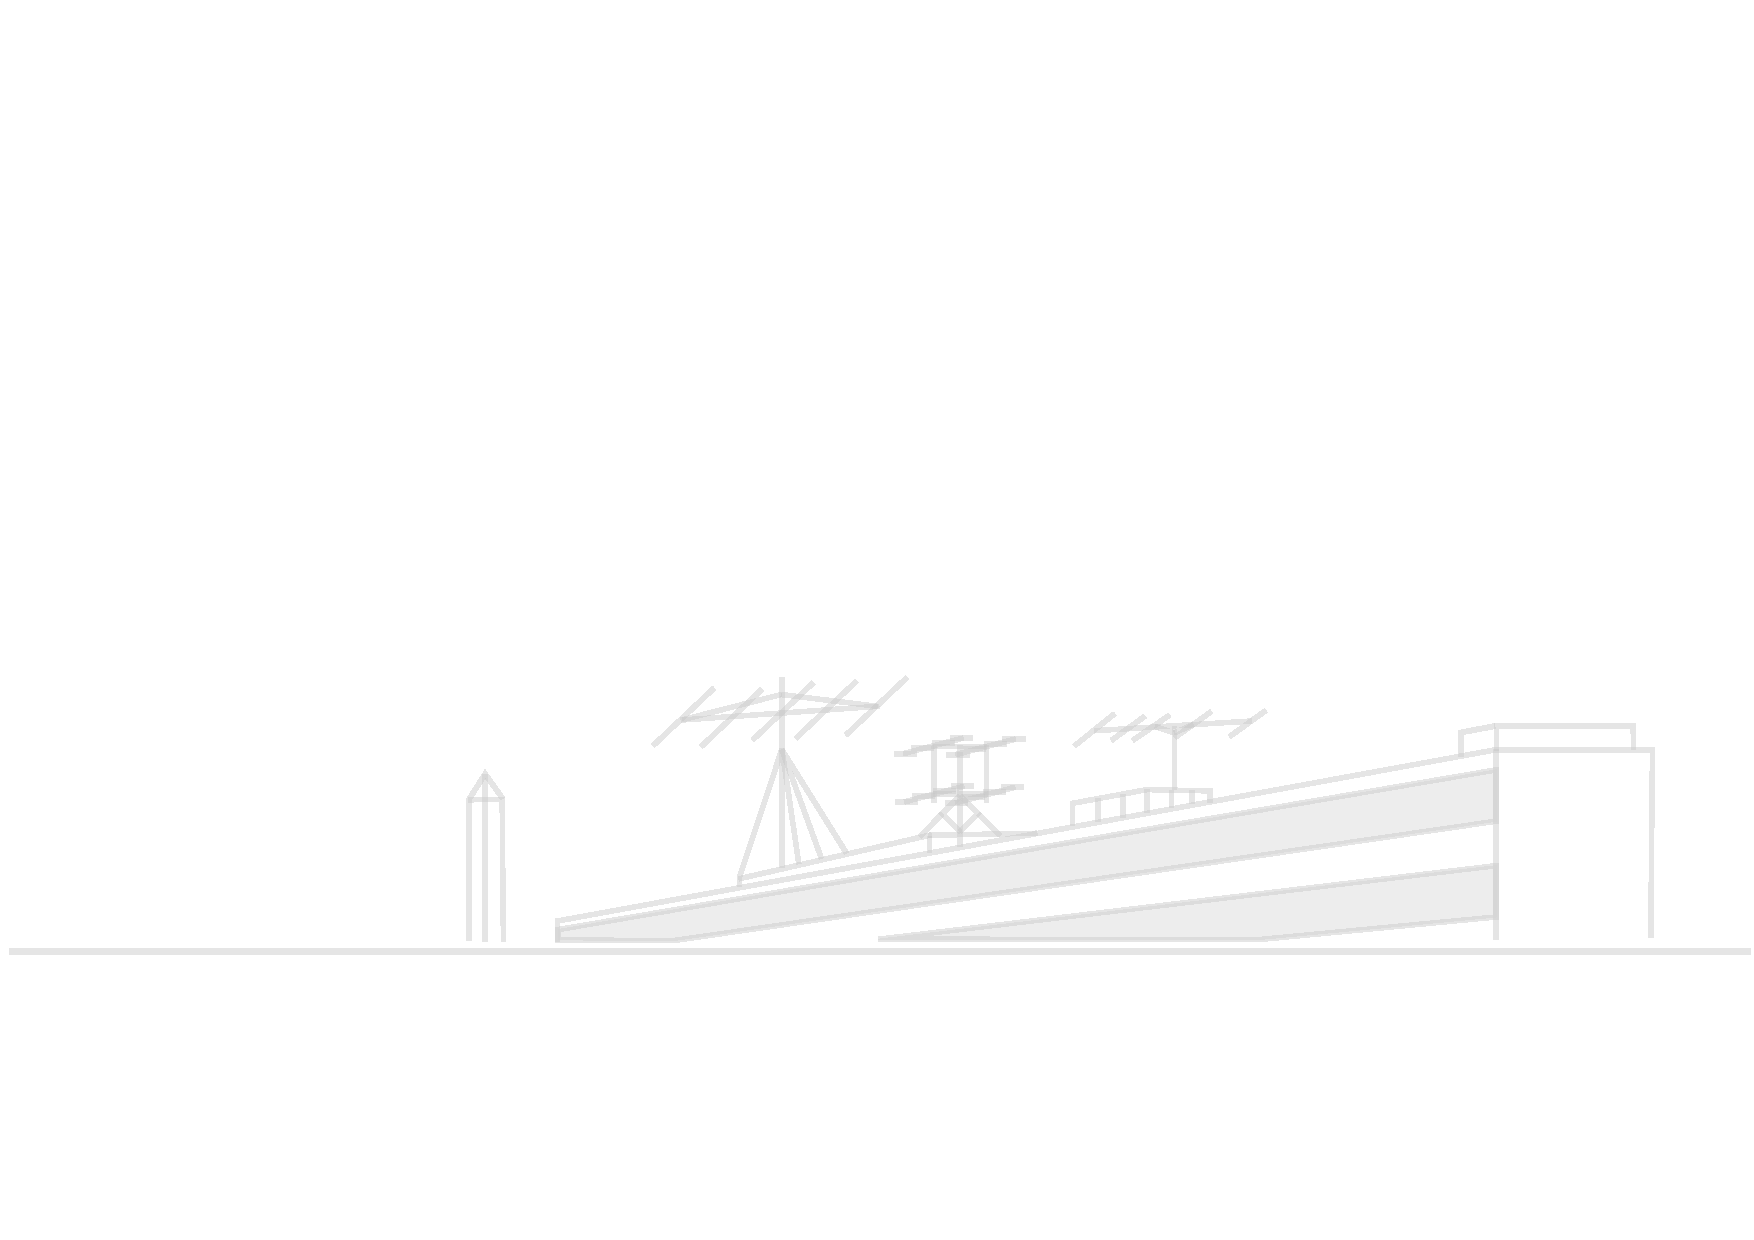
\includegraphics[width=17.8cm]{texdata/dk0tu_rooftop_background.pdf}
}

% Foliennummer einfügen
\setbeamertemplate{footline}[frame number]
%\setbeamertemplate{footline}{}

% Ändere das Zeichen vor jedem item
%\setbeamertemplate{itemize item}{\color{craneorange}$\blacktriangleright$}
%\setbeamertemplate{itemize subitem}{\color{craneorange}$\triangleright$}
%\setbeamertemplate{itemize subsubitem}{\color{craneorange}$\blacktriangleright$}

% Ändert die Blöcke 
\setbeamertemplate{blocks}[rounded][shadow=true]
% default | rounded [shadow=true|false]

%
% Eigene Kommandos
%

% Hack to get natbib and beamer working together. "The beamer user guide suggests
% that only the manual bibliography entry approach is supported"
% on some system it works out of the box, sometimes you need the hack :-(
% so check it --dl7bst
\ifdefined\newblock
    \relax
\else
    \newcommand{\newblock}{}
\fi

% \includedia command to generate png out of a dia file
% NEEDS installed dia and pdflatex option --shell-escape
\newcommand{\includedia}[1]{
    \immediate\write18{/usr/bin/dia #1.dia -e #1_diatmp.png -t png}
}

% RICHIG GROSSER FONT!
\newfont{\bigfont}{cmr10 at 144pt}
\newfont{\smallfont}{cmr10 at 8pt}

% Römische Ziffern
\makeatletter
\newcommand{\rmnum}[1]{\romannumeral #1}
\newcommand{\Rmnum}[1]{\expandafter\@slowromancap\romannumeral #1@}
\makeatother

% Schwarze Überschrift
%\setbeamercolor{frametitle}{fg=black}
%\setbeamercolor{title}{fg=black}

% Item- und Box-Farben
\definecolor{deepBlue}{HTML}{000066}
\setbeamercolor{itemize item}{fg=deepBlue}
\setbeamercolor{itemize subitem}{fg=deepBlue}
\setbeamercolor{description item}{fg=deepBlue}
\setbeamercolor{block title}{fg=deepBlue!100, bg=blue!15}
\setbeamercolor{block body}{fg=black, bg=blue!5}
\setbeamercolor{block title alerted}{fg=deepBlue, bg=red!75}
\setbeamercolor{block body alerted}{fg=black, bg=red!15}
\setbeamercolor*{block title example}{fg=blue!50, bg=blue!10}
\setbeamercolor*{block body example}{fg= blue, bg=blue!5}

%\setbeamercolor{section in head/foot}{parent=palette primary}
%\setbeamercolor{subsection in head/foot}{parent=palette secondary}
%\setbeamercolor{sidebar}{fg=darkblue,bg=yellow!90!orange}
%\setbeamercolor{title in sidebar}{fg=darkblue}
%\setbeamercolor{author in sidebar}{fg=darkblue}
%\setbeamercolor{section in sidebar}{fg=darkblue!10!black}
%\setbeamercolor{subsection in sidebar}{fg=darkblue!50!black}

% Titlepage Infos
\title{AFu-Kurs nach DJ4UF}
\author[DKØTU]{DKØTU\\ \footnotesize{Amateurfunkgruppe der TU Berlin}}
\institute[DKØTU]{\url{http://www.dk0tu.de} }

% PDF-Eigenschaften
\subject{DK0TU-Amateurfunkkurs nach DJ4UF}
\keywords{Amateurfunk Kurs HAM Radio Course CC-BY-NC-SA OpenSource TU Berlin DK0TU}

\subtitle{Technik Klasse A 06: \\
          Transistor \& Verstärker \\[2em]}
\date{Stand 04.05.2016}
 \begin{document}

\begin{frame}
    \titlepage
    \vfill
    \begin{center}
        \ccbyncsaeu\\
        {\tiny This work is licensed under the \em{Creative Commons Attribution-NonCommercial-ShareAlike 3.0 License}.}\\[0.5ex]
         \tiny Amateurfunkgruppe der Technische Universität Berlin (AfuTUB), DKØTU
         %\includegraphics[scale=0.5]{img/DK0TU_Logo.pdf}
    \end{center}
\end{frame}


%FIXME Referenzen/Fußnoten-Systematik vereinheitlichen
%FIXME Abbildungsnummern nicht hard coded

\section*{Aufbau}

\begin{frame}
\frametitle{Bipolarer Transistor}
\begin{minipage}{0.4\textwidth}
	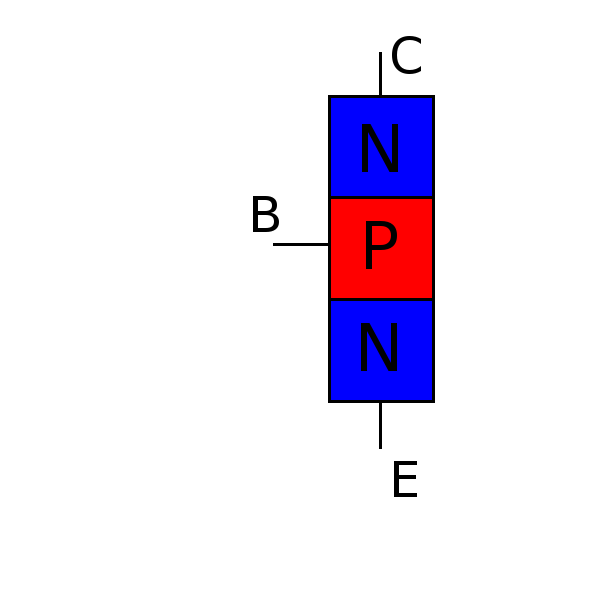
\includegraphics[width=\textwidth,height=.5\textheight,keepaspectratio]{a06/NPN_hlb.png}\\
	{\tiny Abb.\,1: Schichten eines NPN-Transistors}
\end{minipage}
\hspace{0.5cm}
\begin{minipage}{0.4\textwidth}
	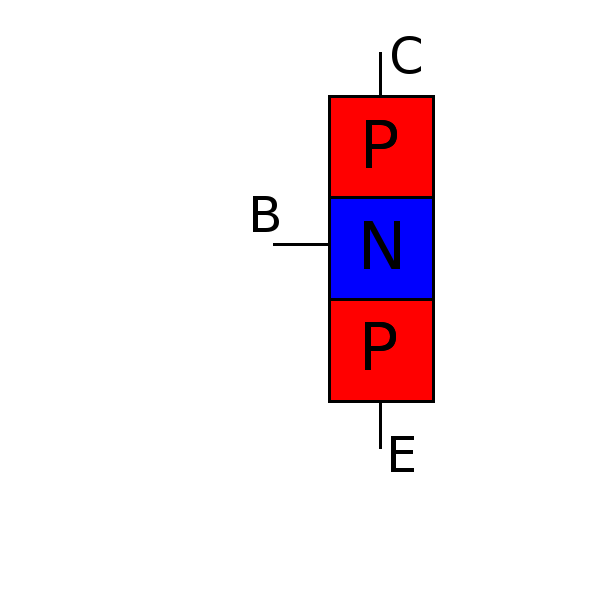
\includegraphics[width=\textwidth,height=.5\textheight,keepaspectratio]{a06/PNP_hlb.png}\\
	{\tiny Abb.\,2: Schichten eines PNP-Transistors}
\end{minipage}
\vspace{0.5cm}
\begin{center}
\begin{itemize}
	\item Transistoren bestehen aus drei Halbleiterschichten
	\item Anschlüsse: Basis (B), Kollektor (C), Emitter (E)
\end{itemize}
\end{center}
\end{frame}

\begin{frame}
\frametitle{Ersatzschaltbild}
\begin{minipage}{0.4\textwidth}
	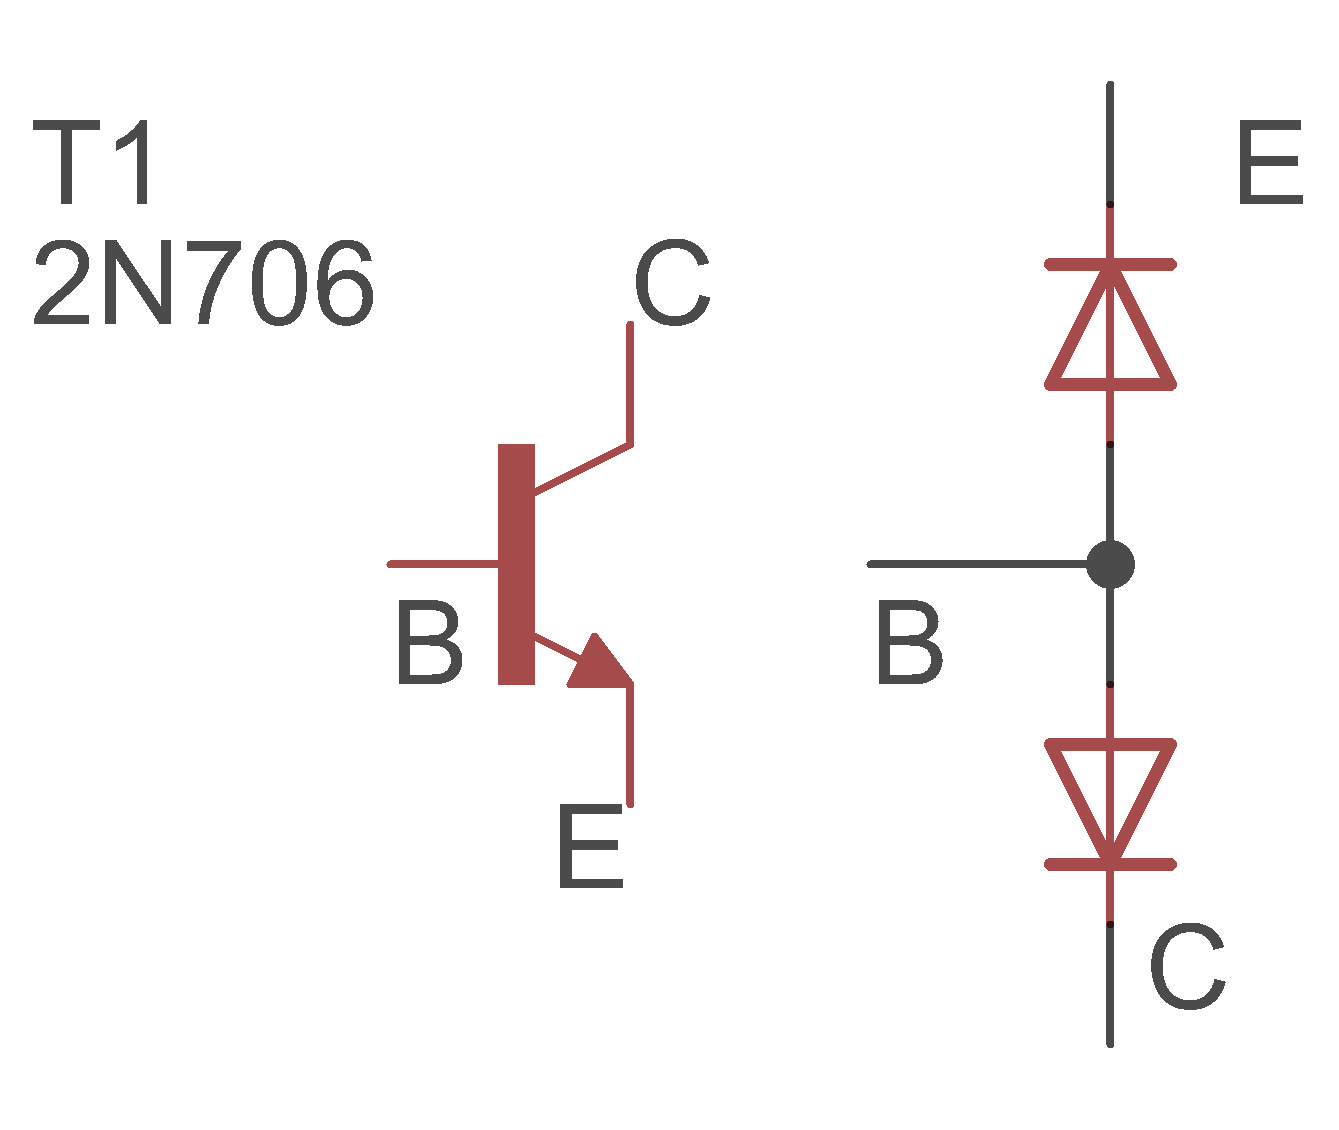
\includegraphics[width=\textwidth,height=.5\textheight,keepaspectratio]{a06/NPN_esb.png}\\
	{\tiny Abb.\,3: ESB eines NPN-Transistors}
\end{minipage}
\hspace{0.5cm}
\begin{minipage}{0.4\textwidth}
	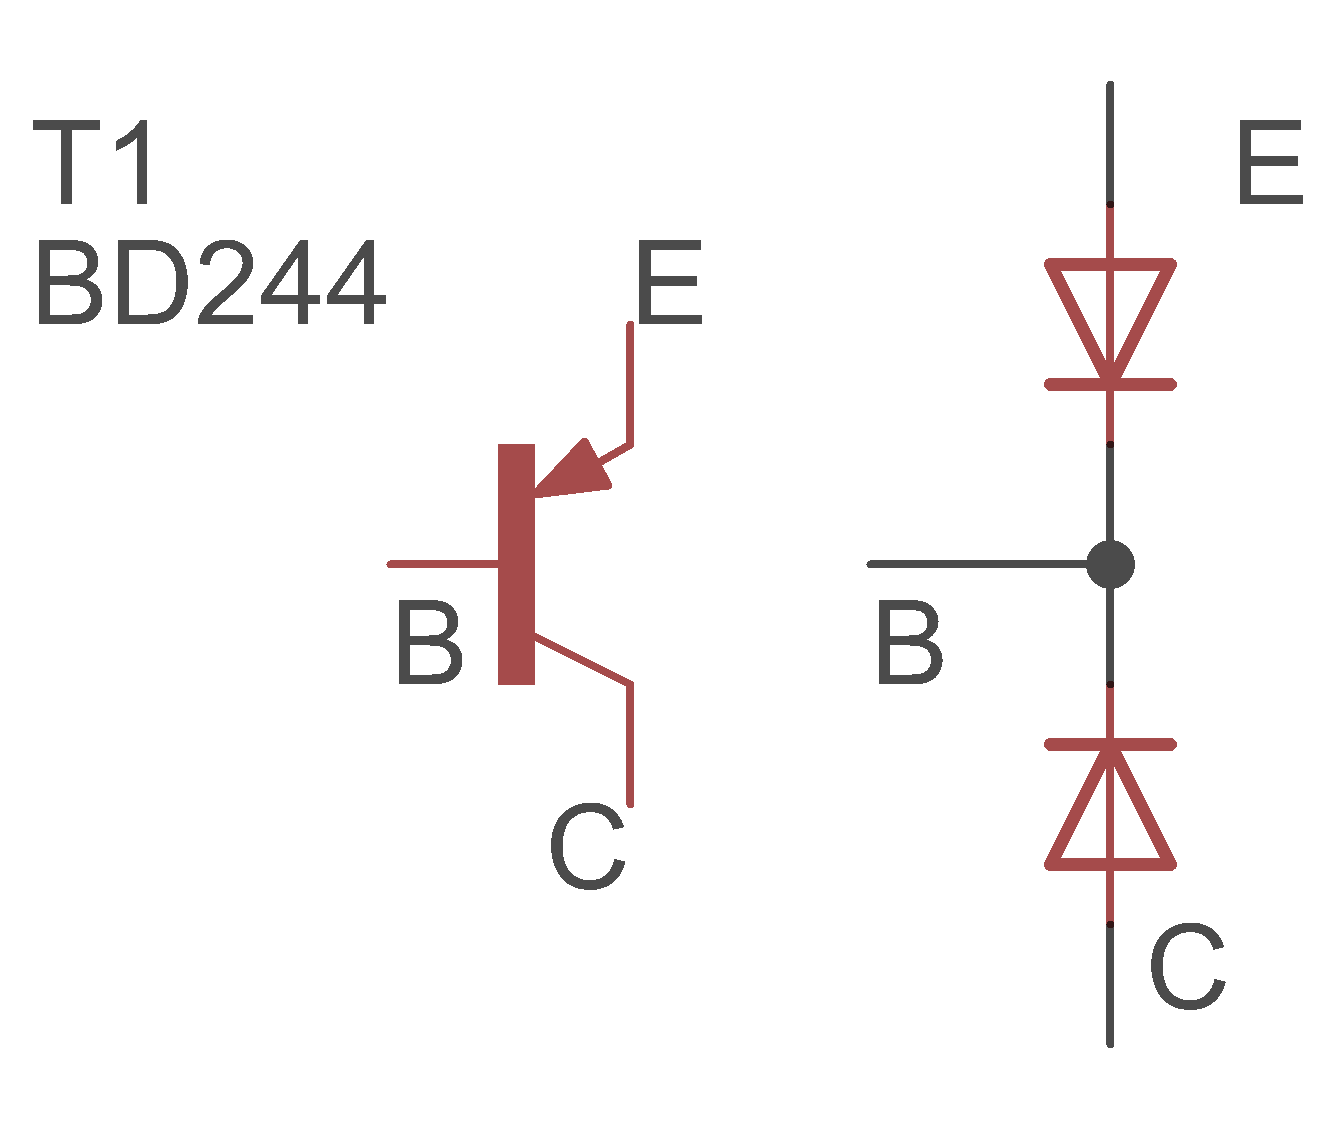
\includegraphics[width=\textwidth,height=.5\textheight,keepaspectratio]{e13/PNP_esb.png}\\
	{\tiny Abb.\,4: ESB eines PNP-Transistors}
\end{minipage}
\vspace{2mm}
\begin{itemize}
	\item	Basis-Emitterübergang muss in Durchlassrichtung gepolt sein
	\item	Basis braucht ein um etwa 0,6 V höheres Potential als der Emitter
\end{itemize}

\end{frame}


\section*{FET}
\begin{frame}
\frametitle{Feldeffekt Transistor (FET)}
\begin{center}
	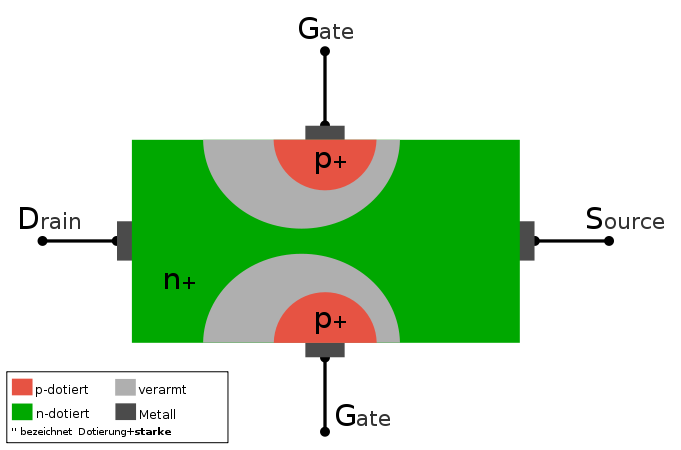
\includegraphics[width=\textwidth,height=.6\textheight,keepaspectratio]{a06/FET-aufbau.png}\\
	{\tiny Abb.\,5: Aufbau eines J-FET~\cite{wp}}
\begin{itemize}
	\item Gate steuert Kanalbreite durch Spannung
	\item Je dünner der Kanal, desto höher ist der Kanalwiderstand
\end{itemize}
\end{center}
\end{frame}

\begin{frame}
	\begin{center}
		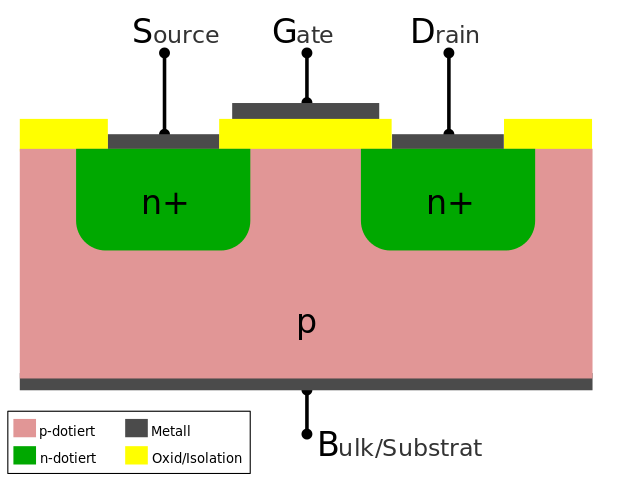
\includegraphics[width=\textwidth,height=.85\textheight,keepaspectratio]{a06/Isolierschicht-FET-intern.png}\\
		{\tiny Abb.\,6: MOSFET in Planartechnologie~\cite{wmde}}
	\end{center}
\end{frame}

\begin{frame}
\frametitle{Weitere FET-Arten}
\begin{center}
	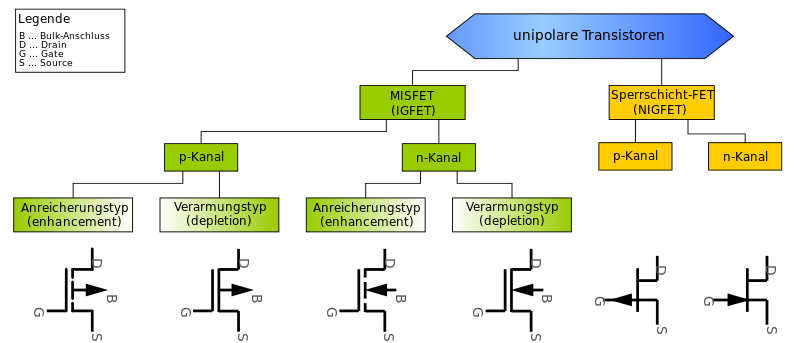
\includegraphics[width=\textwidth,height=.8\textheight,keepaspectratio]{a06/FET-overview.png}\\
	{\tiny Abb.\,7: Übersicht über FETs~\cite{wp}}
\end{center}
\end{frame}

\begin{frame}
	\begin{center}
		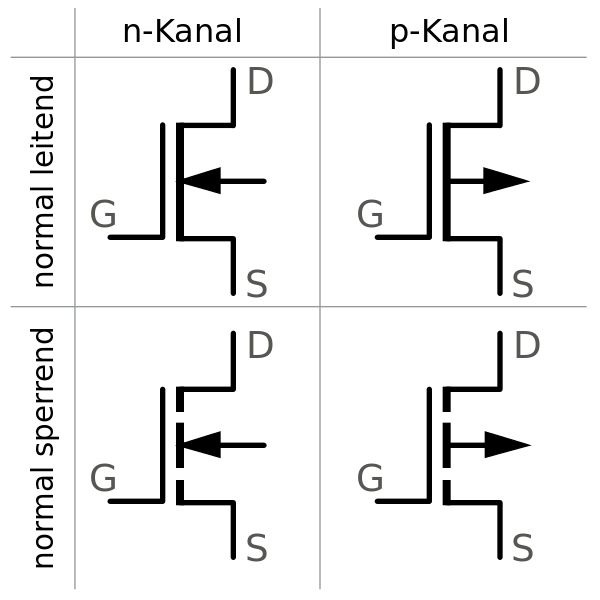
\includegraphics[width=\textwidth,height=.85\textheight,keepaspectratio]{a06/MOSFET-Symbole.png}\\
		{\tiny Abb.\,8: Schaltzeichen des MOSFETS~\cite{wmde}}
	\end{center}
\end{frame}

\begin{frame}
	\begin{center}
		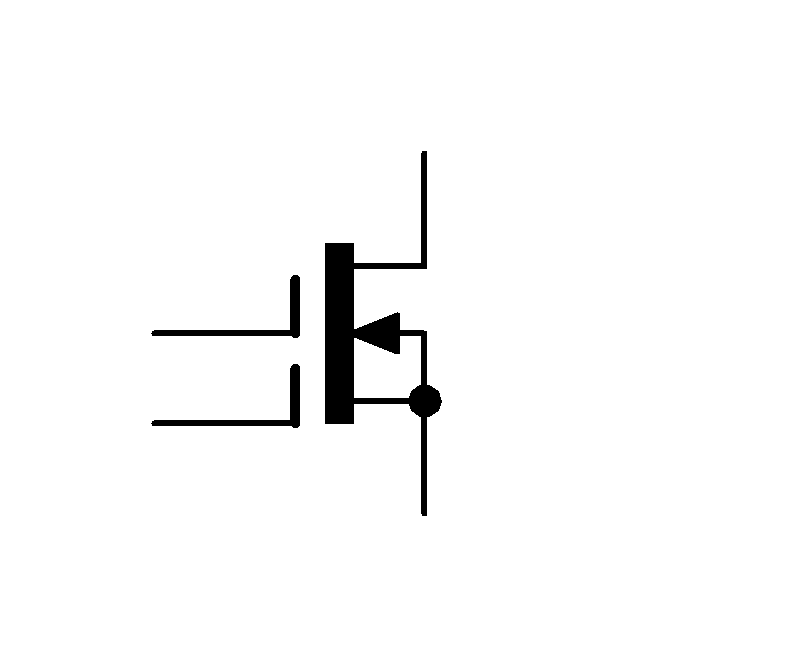
\includegraphics[width=\textwidth,height=.6\textheight,keepaspectratio]{a06/Dual-Gate-MOSFET.png}\\
		{\tiny Abb.\,9: Schaltzeichen eines Dual-Gate-MOSFETs}
	\end{center}
	\begin{itemize}
		\item Besitzt zwei Gateanschlüsse
		\item Wird für Mischerschaltungen genutzt
	\end{itemize}
\end{frame}

\begin{frame}
  \begin{tabular}{p{2.5pc}||c||p{2.5pc}||c}\hline
    \textbf{TC604} & \multicolumn{3}{p{.8\textwidth}}{\textbf{Welcher der folgenden Transistoren ist ein selbstleitender P"~Kanal MOSFET}} \\ \hline\hline
    A & 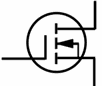
\includegraphics[width=.35\textwidth,height=.35\textheight,keepaspectratio]{a06/tc604c.png} &
    B & 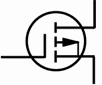
\includegraphics[width=.35\textwidth,height=.35\textheight,keepaspectratio]{a06/tc604d.png} \\ \hline
    C \only<2>\checkmark & 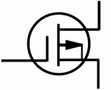
\includegraphics[width=.35\textwidth,height=.35\textheight,keepaspectratio]{a06/tc604a.png} &
    D & 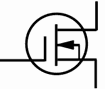
\includegraphics[width=.35\textwidth,height=.35\textheight,keepaspectratio]{a06/tc604b.png} \\ \hline
  \end{tabular}
\end{frame}

\begin{frame}
  \begin{tabular}{p{2.5pc}||c||p{2.5pc}||c}\hline
    \textbf{TC605} & \multicolumn{3}{p{.8\textwidth}}{\textbf{Welcher der folgenden Transistoren ist ein selbstsperrender N"~Kanal MOSFET}} \\ \hline\hline
    A \only<2>\checkmark & 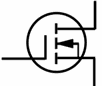
\includegraphics[width=.35\textwidth,height=.35\textheight,keepaspectratio]{a06/tc604c.png} &
    B & 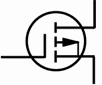
\includegraphics[width=.35\textwidth,height=.35\textheight,keepaspectratio]{a06/tc604d.png} \\ \hline
    C & 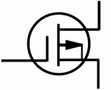
\includegraphics[width=.35\textwidth,height=.35\textheight,keepaspectratio]{a06/tc604a.png} &
    D & 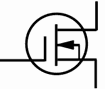
\includegraphics[width=.35\textwidth,height=.35\textheight,keepaspectratio]{a06/tc604b.png} \\ \hline
  \end{tabular}
\end{frame}


\section*{Bipolar\-transistor}
\begin{frame}
  \frametitle{Anwendungen von Bipolartransistoren}
	\begin{minipage}{0.4\textwidth}
		\begin{center}
			{\Large Schalter}
			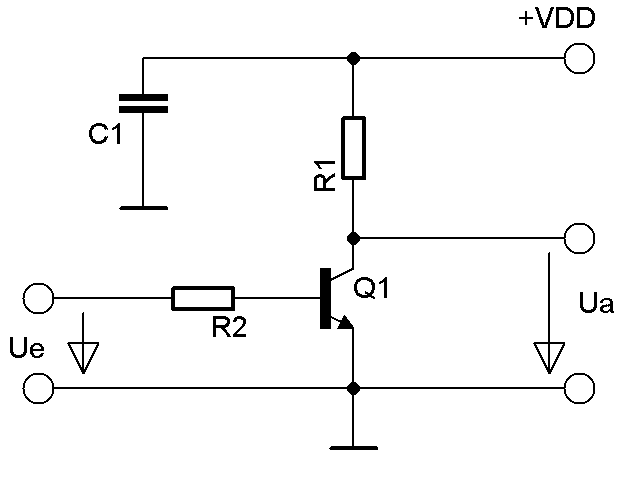
\includegraphics[width=\textwidth,height=.7\textheight,keepaspectratio]{a06/Transistor-Schalter.png}\\
		\end{center}	
	\end{minipage}
	\hspace{3mm}
	\begin{minipage}{0.4\textwidth}
		\begin{center}
			{\Large Verstärker}
			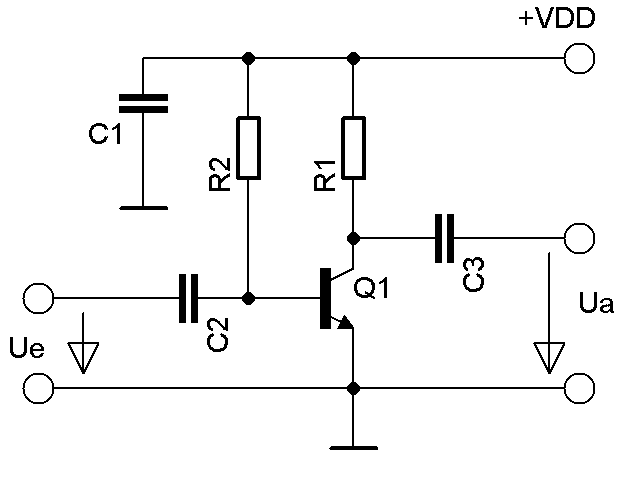
\includegraphics[width=\textwidth,height=.7\textheight,keepaspectratio]{a06/Transistor-Verstaerker.png}\\
		\end{center}	
	\end{minipage}\\
	\vspace{3mm}
	{\tiny Abb.\,10: Anwendungen von Transistoren~\cite{bnetza}}
	\begin{itemize}
		\item	Transistoren können als Schalter oder als Verstärker genutzt werden
	\end{itemize}
\end{frame}

\section*{Anwendungen}
\subsection*{Transistor als Schalter}
\begin{frame}
	\frametitle{Transistor als Schalter}
	\begin{minipage}{0.4\textwidth}
	\begin{center}
			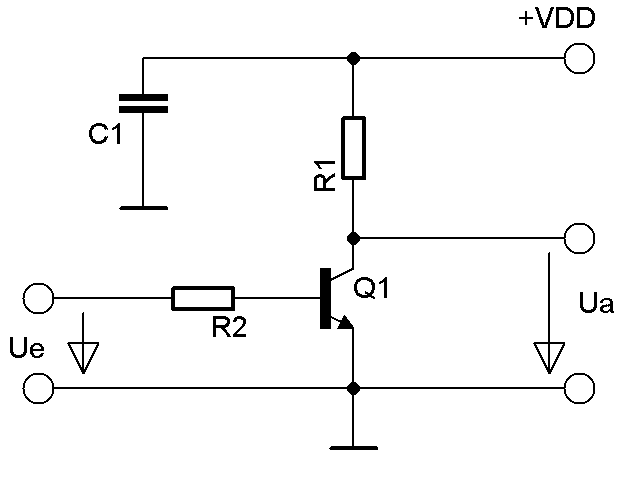
\includegraphics[width=\textwidth,height=.85\textheight,keepaspectratio]{a06/Transistor-Schalter.png}\\
			{\tiny Abb.\,11: Transistor als Schalter mit Belastung gegen Masse~\cite{bnetza}}
		\end{center}
	      \end{minipage}
	      \hspace{3mm}
	      \begin{minipage}{0.5\textwidth}
		\begin{itemize}
			\item $U_e = 0 V \rightarrow$ Transistor sperrt\\ $\rightarrow U_a = U_B$\\ $\Rightarrow$ Eingang 0, Ausgang 1
			\item $U_e \gg 0,6 V \rightarrow$ Transistor leitet\\ $\rightarrow U_a \approx 0.1 V$\\ $\Rightarrow$ Eingang 1, Ausgang 0
			\item Der Transistor erfüllt hier die Funktion eines \textbf{Inverters}
		\end{itemize}
	      \end{minipage}
\end{frame}

\begin{frame}
	\frametitle{Transistor mit Koppelkondensator als Schalter}
	\begin{minipage}{0.4\textwidth}
	\begin{center}
			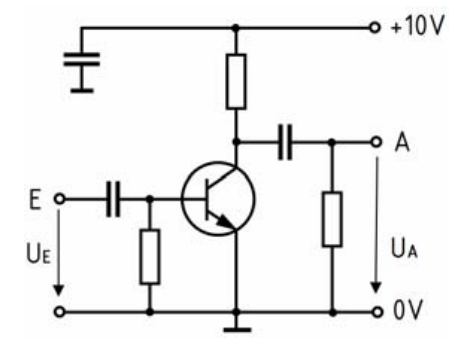
\includegraphics[width=\textwidth,height=.85\textheight,keepaspectratio]{a06/Transistor-Schalter+C.png}\\
			{\tiny Abb.\,12: Transistor mit Koppelkondensator als Schalter~\cite{bnetza}}
		\end{center}
	      \end{minipage}
	      \hspace{3mm}
	      \begin{minipage}{0.5\textwidth}
		\begin{itemize}
			\item	Der Kondensator blockt die Gleichspannung und bildet den Mittelwert der Wechselspannung
		\end{itemize}
	      \end{minipage}
\end{frame}

\begin{frame}
  \begin{tabular}{p{2.5pc}||l||p{2.5pc}||l}\hline
    \textbf{TD431} & \multicolumn{3}{p{.8\textwidth}}{
    \begin{tabular}{c}
      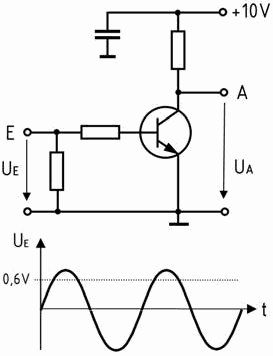
\includegraphics[width=\textwidth,height=.45\textheight,keepaspectratio]{a06/td431.png}
    \end{tabular}
    \begin{tabular}{p{.55\textwidth}}
      \textbf{An den Eingang dieser Schaltung wird das folgende Signal gelegt. Welches ist ein mögliches Ausgangssignal $U_A$?}
    \end{tabular}
     } \\ \hline\hline
    A & 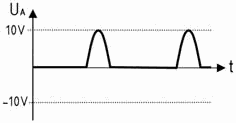
\includegraphics[width=.25\textwidth,height=.25\textheight,keepaspectratio]{a06/td431d.png} &
    B & 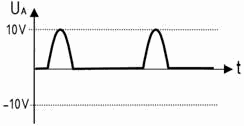
\includegraphics[width=.25\textwidth,height=.25\textheight,keepaspectratio]{a06/td431c.png} \\ \hline
    C & 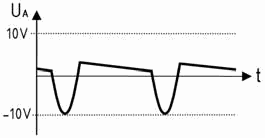
\includegraphics[width=.25\textwidth,height=.25\textheight,keepaspectratio]{a06/td431b.png} &
    D \only<2>\checkmark & 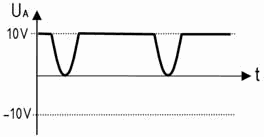
\includegraphics[width=.25\textwidth,height=.25\textheight,keepaspectratio]{a06/td431a.png} \\ \hline
  \end{tabular}
\end{frame}

\begin{frame}
  \begin{tabular}{p{2.5pc}||l||p{2.5pc}||l}\hline
    \textbf{TD432} & \multicolumn{3}{p{.8\textwidth}}{
    \begin{tabular}{c}
      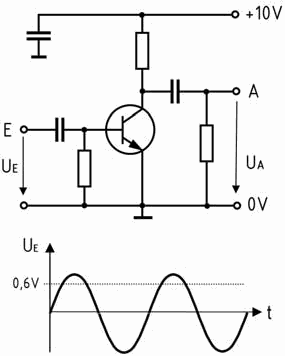
\includegraphics[width=\textwidth,height=.45\textheight,keepaspectratio]{a06/td432.png}
    \end{tabular}
    \begin{tabular}{p{.55\textwidth}}
      \textbf{An den Eingang dieser Schaltung wird das folgende Signal gelegt. Welches ist ein mögliches Ausgangssignal $U_A$?}
    \end{tabular}
     } \\ \hline\hline
    A & 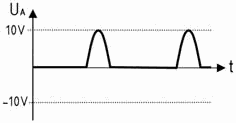
\includegraphics[width=.25\textwidth,height=.25\textheight,keepaspectratio]{a06/td431d.png} &
    B & 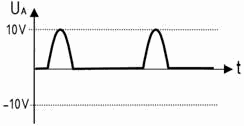
\includegraphics[width=.25\textwidth,height=.25\textheight,keepaspectratio]{a06/td431c.png} \\ \hline
    C \only<2>\checkmark & 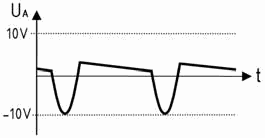
\includegraphics[width=.25\textwidth,height=.25\textheight,keepaspectratio]{a06/td431b.png} &
    D & 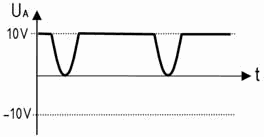
\includegraphics[width=.25\textwidth,height=.25\textheight,keepaspectratio]{a06/td431a.png} \\ \hline
  \end{tabular}
\end{frame}


\begin{frame}
	\frametitle{Transistor als Schalter mit Überspannungsschutzdiode}
	\begin{minipage}{0.4\textwidth}
	\begin{center}
		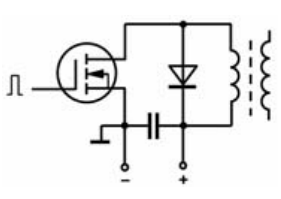
\includegraphics[width=\textwidth,height=.85\textheight,keepaspectratio]{a06/Transistor-Schalter+L.png}\\
		{\tiny Abb.\,13: Transistor als Schalter einer Induktiven Last~\cite{bnetza}}
	\end{center}
      \end{minipage}
      \hspace{3mm}
      \begin{minipage}{0.5\textwidth}
	\begin{itemize}
		\item Durch plötzliches Abschalten baut sich eine hohe Induktionsspannung auf
		\item Diese kann den Transistor zerstören
		\item Um das zu verhindern wird eine Diode parallel zur Spule eingebaut
		\item Diese führt die Induktionsspannung an dem Transistor vorbei ab
	\end{itemize}
      \end{minipage}
\end{frame}

% \begin{frame}
%   \begin{tabular}{p{2.5pc}||c||p{2.5pc}||c}\hline
%     \textbf{TC528} & \multicolumn{3}{p{.8\textwidth}}{\textbf{In welcher der folgenden Schaltungen ist die Diode zur Spannungsbegrenzung einer Schaltstufe richtig eingesetzt?}} \\ \hline\hline
%     A \only<2>\checkmark & 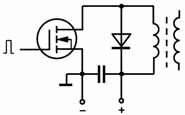
\includegraphics[width=.35\textwidth,height=.35\textheight,keepaspectratio]{a06/tc528a.png} &
%     B & 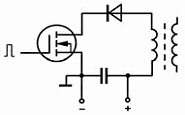
\includegraphics[width=.35\textwidth,height=.35\textheight,keepaspectratio]{a06/tc528d.png} \\ \hline
%     C & 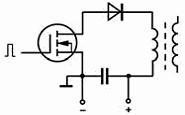
\includegraphics[width=.35\textwidth,height=.35\textheight,keepaspectratio]{a06/tc528c.png} &
%     D & 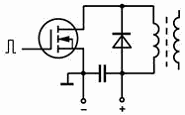
\includegraphics[width=.35\textwidth,height=.35\textheight,keepaspectratio]{a06/tc528b.png} \\ \hline
%   \end{tabular}
% \end{frame}

\subsection*{Verstärker}
\begin{frame}
\frametitle{Verstärker}
\begin{block}{Definition eines Verstärkers nach Captain Obvious}
  \begin{Large}
    Es ist nur dann eine Verstärkung, wenn die Leistung am Ausgang größer ist, als die am Eingang
  \end{Large}
\end{block}
\end{frame}

\begin{frame}
  \frametitle{Transistor als Verstärker in Emitterschaltung}
  \begin{columns}
    \column{.4\textwidth}
    \centering
    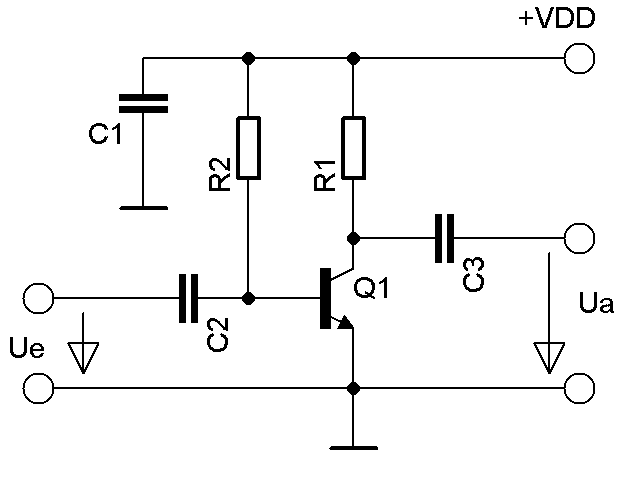
\includegraphics[width=\textwidth,height=.85\textheight,keepaspectratio]{a06/Transistor-Verstaerker.png}\\
    {\tiny Abb.\,14: Transistor als Spannungsverstärker~\cite{bnetza}}
    \only<1>{
    \column{.5\textwidth}
    \begin{itemize}
      \item Benötigt einen richtig eingestellten Arbeitspunkt, um vernünftig zu funktionieren
      \item Dazu wird die Basis"=Emitter"=Spannung $U_{BE}$ auf einen definierten Wert größer $0,6 V$ gesetzt
    \end{itemize}
    }
    \only<2>{
    \column{.5\textwidth}
    \begin{itemize}
      \item Dem durch den Arbeitspunkt eingestellten Ruhestrom überlagert sich die eingekoppelte Wechselspannung
      \item Dadurch wird der Kollektorstrom je nach Eingangsgröße größer oder kleiner
      \item Da der Bipolartransistor nur den Strom verstärkt, wird die Stromverstärkung mittels eines Widerstandes $R_1$ in eine Spannungsverstärkung umgewandelt
    \end{itemize}
    }
    \only<3>{
    \column{.5\textwidth}
    \begin{itemize}
      \item Ändert man die Eingangsspannung $U_e$ der Schaltung, verändert sich auch der Basisstrom
      \item Dies ruft eine Veränderung des Kollektorstromes $I_C$ hervor, die um die Stromverstärkung des Transistors größer ist als der Basisstrom
      \item Die Spannung über $R_1$ verhält sich bei Änderungen genauso wie der Kollektorstrom $I_C$
      \item Dadurch sinkt die Kollektorspannung $U_{CE}$ des Transistors
    \end{itemize}
    }
    \only<4>{
    \column{.5\textwidth}
    \begin{itemize}
      \item Die Kondensatoren $C_2$ und $C_3$ entkoppeln das Eingangs- und das Ausgangssignal
      \item Dadurch wird der Gleich\-spannungs\-anteil entfernt, um das Signal beispielsweise einer weiteren Verstärkerstufe zuzuführen
    \end{itemize}
    }
  \end{columns}
\end{frame}

\begin{frame}
  \begin{tabular}{p{2.5pc}||l||p{2.5pc}||l}\hline
    \textbf{TC626} & \multicolumn{3}{p{.8\textwidth}}{
    \begin{tabular}{c}
      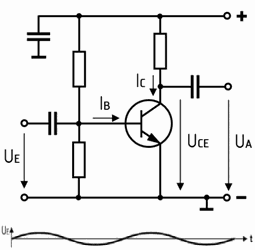
\includegraphics[width=\textwidth,height=.45\textheight,keepaspectratio]{a06/tc626.png}
    \end{tabular}
    \begin{tabular}{p{.48\textwidth}}
      \textbf{Folgendes Signal $U_E$ wurde auf den Eingang folgender Schaltung gegeben. In welcher Antwort sind alle dargestellten Signale phasenrichtig zugeordnet?}
    \end{tabular}
    } \\ \hline\hline
    A & 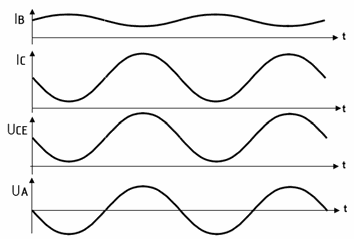
\includegraphics[width=.25\textwidth,height=.25\textheight,keepaspectratio]{a06/tc626c.png} &
    B \only<2>\checkmark & \includegraphics[width=.25\textwidth,height=.25\textheight,keepaspectratio]{a06/tc626a.png} \\ \hline
    C & \includegraphics[width=.25\textwidth,height=.25\textheight,keepaspectratio]{a06/tc626d.png} &
    D & \includegraphics[width=.25\textwidth,height=.25\textheight,keepaspectratio]{a06/tc626b.png} \\ \hline
  \end{tabular}
\end{frame}

\begin{frame}
	\frametitle{Verstärkungen eines Transistors bei Wechselstrom}
	\centering
	\begin{block}{Spannungsverstärkung}
	  $v_U = \cfrac{\Delta U_{CE}}{\Delta U_{BE}}$
	\end{block}

	\begin{block}{Stromverstärkung}
	  $v_I = \beta = \cfrac{\Delta I_C}{\Delta I_B}$
	\end{block}

	\begin{block}{Leistungsverstärkung}
	  $v_P = v_U \cdot v_I$
	\end{block}
\end{frame}


\subsection*{Basisvorspannung}
\begin{frame}
  \frametitle{Generieren der Basisvorspannung}
	\begin{center}
		\includegraphics[width=.4\textwidth,height=.85\textheight,keepaspectratio]{a06/Transistor-Verstaerker.png}
		\vspace{3mm}
		\includegraphics[width=.4\textwidth,height=.85\textheight,keepaspectratio]{a06/Transistor-Verstaerker-C.png}\\
		{\tiny Abb.\,17: Möglichkeiten die Basisvospannung zu erzeugen}
	\end{center}
\end{frame}

\begin{frame}
	\frametitle{Basisvorspannung, warum eigentlich?}
	\begin{itemize}
		\item Will man eine Wechselspannung verstärken, muss man den Mittelpunkt des Signals in den Aussteuerbereich verschieben
		\item Da sonst die obere oder untere Halbwelle nicht originalgetreu wiedergegeben wird
		\item Dazu überlagert man die Wechselspannung mit einer mittleren Gleichspannung
		\item Das Erzeugen der mittleren Gleichspannung nennt man einstellen des Arbeitspunktes oder der Basisvorspannung
	\end{itemize}
\end{frame}

\begin{frame}
  % https://de.wikipedia.org/wiki/Arbeitspunkt#/media/File:Arbeitspunkt.PNG
  \includegraphics[width=\textwidth,height=\textheight,keepaspectratio]{a06/Arbeitspunkt.png}\\
  {\tiny Abb.\,30: Arbeitspunkteinstellung~\cite{wp}}
\end{frame}

\begin{frame}
  \frametitle{Einstellen des Arbeitspunktes}
  \begin{columns}
    \column{.5\textwidth}
    \includegraphics[width=\textwidth,height=.85\textheight,keepaspectratio]{a06/Kombiniertes_Kennlinienfeld_Transistor_2.pdf}
    {\tiny Abb.\,31: Vierquadrantenkennlinienfeld \cite{wp}}
    \column{.45\textwidth}
    \begin{itemize}
	\only<1>{
      \item Will man den Arbeitspunkt eines Transistors mit der Vorspannung einstellen, muss man zwei Spannungen dimensionieren
      \item Zum einen muss die Basisspannung eingestellt werden und zum anderen die Kollektorspannung
      \item Die Kollektorspannung bestimmen wir, indem wir einen Spannungsteiler über $R_1$ und dem Kollektor"=Emitter"=Widerstand $R_{CE}$ (Lastwiderstand) berechnen
	}
	\only<2>{
      \item Für eine symmetrische Aussteuerung nehmen wir an, dass sowohl über $R_1$ als auch über $R_{CE}$  $\frac{V_{DD}}{2}$ anliegen
      \item Danach wählt man einen Kollektorstrom den der Transistor verkraften kann
      \item Dann berechnet man mittels Ohmschen Gesetz den Widerstand $R_1$
	}
	\only<3>{
      \item Um die Basisvorspannung zu erzeugen, gibt es zwei Möglichkeiten:
	\begin{itemize}
	  \item mit einem Widerstand
	  \item mit einem Spannungsteiler (siehe Abb.\,17)
	\end{itemize}
	}
    \end{itemize}
  \end{columns}
\end{frame}

\begin{frame}
	\frametitle{Arbeitspunktstabilisierung durch Stromgegenkopplung}
	\begin{minipage}{0.4\textwidth}
	\begin{center}
		\includegraphics[width=\textwidth,height=.85\textheight,keepaspectratio]{a06/Transistor-Verstaerker-APstab1.png}\\
		{\tiny Abb.\,18: Transistor als Spannungsverstärker~\cite{bnetza}}
	\end{center}
      \end{minipage}
      \hspace{3mm}
      \begin{minipage}{0.5\textwidth}
        % $U_2$ = konstant
        % $I_C$ steigt $\rightarrow I_E$ steigt $\rightarrow U_{R3}$ steigt $\rightarrow U_{R2} = U_{R3} + U_{BE} \rightarrow U_{BE}$ sinkt $\rightarrow $Transistor sperrt$ \rightarrow I_C sinkt$
	    \begin{itemize}
	        \item Der Transistor ist nicht temperaturstabil, was zum Anstieg von $I_B$ und damit $I_C$ und $I_E$ führt
	        \item $U_{R3}$ steigt und $U_{BE}$ sinkt
	        \item Bei kleinerer $U_{BE}$ sinkt $I_B$ und damit $I_C$ und $I_E$
	        \item Die Spannung $U_{R3}$ wird wieder kleiner und $U_{BE}$ wieder größer
	    \end{itemize}
      \end{minipage}
\end{frame}

\begin{frame}
	\begin{itemize}
		\item Querstrom $I_{quer}$ durch $R_2$ wird 3 bis 10 mal so groß wie der
              Basisstrom dimensioniert: \\
		
        $I_{quer} = 3 ... 10 \cdot I_B$
		
        \item Kondensator am Emitter überbrückt Wechselstromsignale
        \begin{itemize}
		    \item dadurch werden Verstärkungsverluste bei höheren Frequenzen aufgehoben
            \item baut man am Emitter keinen Kondensator ein, fällt die Verstärkung des
                  Transistors stark ab \& liegt dann bei dem Verhältnis aus Kollektor- zu
                  Emitterwiderstand
        \end{itemize}
	\end{itemize}
\end{frame}

\begin{frame}
    \frametitle{Arbeitspunktstabilisierung durch Spannungsgegenkopplung}
	\begin{center}
		\includegraphics[width=.4\textwidth,height=.85\textheight,keepaspectratio]{a06/Transistor-Verstaerker-APstab2a.png}
		\vspace{3mm}
		\includegraphics[width=.4\textwidth,height=.85\textheight,keepaspectratio]{a06/Transistor-Verstaerker-APstab2b.png}\\
		{\tiny Abb.\,19: Möglichkeiten zur Arbeitspunktstabilisierung via Spannungsgegenkopplung}
	\end{center}
\end{frame}

\begin{frame}
  \begin{minipage}{0.4\textwidth}
	\begin{center}
		\includegraphics[width=\textwidth,height=.85\textheight,keepaspectratio]{a06/Transistor-Verstaerker-APstab2a.png}\\
		{\tiny Abb.\,20: Transistor als Spannungsverstärker~\cite{bnetza}}
	\end{center}
      \end{minipage}
      \hspace{3mm}
      \begin{minipage}{0.5\textwidth}
	\begin{itemize}
		\item $R_1$ stabilisiert gegen thermischen Einfluss
		\item $I_C$ steigt $\rightarrow U_{CE}$ sinkt $\rightarrow U_{BE}$ sinkt
              $\rightarrow$ Transistor ``sperrt'' $\rightarrow I_C$ sinkt wieder
	\end{itemize}
      \end{minipage}
\end{frame}

\subsection*{Grundschaltungen}
\begin{frame}
	\frametitle{Grundschaltungen des Transistors}
	\begin{small}
	\begin{tabular}{|c|c|c|c|}
	\hline
	" " &Emitterschaltung & Kollektorschaltung & Basisschaltung \\ \hline
	" "     & \includegraphics[width=.3\textwidth,height=.3\textheight,keepaspectratio]{a06/Emitterschaltung.png}
		& \includegraphics[width=.3\textwidth,height=.3\textheight,keepaspectratio]{a06/Kollektorschaltung.png}
		& \includegraphics[width=.3\textwidth,height=.3\textheight,keepaspectratio]{a06/Basisschaltung.png} \\ \hline
	$r_e$ & mittel z.B. $1k\Omega$ & klein z.B. $50\Omega$ & groß z.B. $100k\Omega$ \\ \hline
	$r_a$ & mittel z.B. $10k\Omega$ & groß z.B. $100k\Omega$ & klein z.B. $50\Omega$ \\ \hline
	$v_i$ & groß z.B. $100$ & $<1$ z.B. $0,9$ & groß z.B. $100$ \\ \hline
	$v_u$ & groß z.B. $100$ & groß z.B. $100$ & $<1$ z.B. $0,99$ \\ \hline
	$v_p$ & sehr groß z.B. $1k\Omega$ & groß z.B. $100$ & groß z.B. $100$ \\ \hline
	$\varphi_u$ & gegenphasig $180^{\circ}$ & gleichphasig $0^{\circ}$ & gleichphasig $0^{\circ}$ \\ \hline
	\end{tabular}
	\end{small}
\end{frame}

\begin{frame}
  \begin{exampleblock}{Fakultative Hausaufgabe}
    Prüfungsfragen TC618--TC625, TF321--TF324
  \end{exampleblock}
\end{frame}

\section*{Integierte Schaltung}
\begin{frame}
\frametitle{Integierte Schaltung}
Heutzutage komplexe Schaltungen auf einem Halbleiterkristall
\begin{minipage}{0.3\textwidth}
	\includegraphics[width=\textwidth,height=.6\textheight,keepaspectratio]{a06/IC.jpg}\\
	{\tiny Abb.\,21: IC auf einer Platine~\cite{wp}}
\end{minipage}
\hspace{0.5cm}
\begin{minipage}{0.5\textwidth}
\begin{center}
	\includegraphics[width=\textwidth,height=.6\textheight,keepaspectratio]{a06/IC2.jpg}\\
	{\tiny Abb.\,22: Offener IC~\cite{wpen}}
\end{center}
\end{minipage}
\end{frame}

\section*{Operations\-verstärker}

\begin{frame}
  \frametitle{Operationsverstärker}
  \begin{center}
    \includegraphics[width=\textwidth,height=.85\textheight,keepaspectratio]{a06/OPV-intern.png}\\
    {\tiny Abb.\,23: Innerer Aufbau eines OPVs~\cite{wp}}
  \end{center}
\end{frame}

\begin{frame}
  \frametitle{Invertierender Verstärker}
  \begin{minipage}{0.4\textwidth}
    \begin{center}
      \includegraphics[width=\textwidth,height=.85\textheight,keepaspectratio]{a06/OPV-Inverter.png}\\
      {\tiny Abb.\,24: OPV als invertierender Verstärker}
    \end{center}
  \end{minipage}
  \hspace{2pc}
  \begin{minipage}{0.5\textwidth}
    \centering
    \begin{block}{Invertierender Verstärker}
      $v_u = -\cfrac{U_A}{U_E} = -\cfrac{R_2}{R_1}$
    \end{block}
  \end{minipage}
\end{frame}

\begin{frame}
  \frametitle{Nicht-invertierender Verstärker}
  \begin{minipage}{0.4\textwidth}
    \begin{center}
      \includegraphics[width=\textwidth,height=.85\textheight,keepaspectratio]{a06/OPV-nonInverter.png}\\
      {\tiny Abb.\,25: OPV als nicht-invertierender Verstärker}
    \end{center}
  \end{minipage}
  \hspace{2pc}
  \begin{minipage}{0.5\textwidth}
    \centering
    \begin{block}{Nicht-invertierender Verstärker}
      $v_u = \cfrac{U_A}{U_E} = 1+\cfrac{R_2}{R_1}$
    \end{block}
    Wird häufig als Impedanzwandler eingesetzt
  \end{minipage}
\end{frame}

\begin{frame}
  \frametitle{Impedanzwandler}
  \begin{minipage}{0.4\textwidth}
    \begin{center}
      \includegraphics[width=\textwidth,height=.85\textheight,keepaspectratio]{a06/Impedanzwandler.png}\\
      {\tiny Abb.\,26: OPV als Impedanzwandler}
    \end{center}
  \end{minipage}
  \begin{minipage}{0.5\textwidth}
    \begin{itemize}
      \item Besitzt sehr großen Eingangswiderstand und sehr kleinen Ausgangswiderstand
      \item Ist quasi ein nicht-invertierender Verstärker mit $R_2 = 0 \Omega$ und $R_1 = \infty\Omega$
    \end{itemize}
  \end{minipage}
\end{frame}


\begin{frame}
  \begin{exampleblock}{Fakultative Hausaufgabe}
    Prüfungsfragen TC711--TC717
  \end{exampleblock}
\end{frame}

\section*{Elektronenröhre}

\begin{frame}
	\begin{center}
		\includegraphics[width=\textwidth,height=.5\textheight,keepaspectratio]{a06/Roehren.jpg}\\
		{\tiny Abb.\,27: Verschiedene Elektronenröhren~\cite{wmde}}
	\end{center}
	\begin{itemize}
		\item Arbeiten mit hohen Spannungen und geringen Strömen
		\item Ist ein gepoltes Bauteil
	\end{itemize}
\end{frame}

\begin{frame}
  \frametitle{Die Röhre}
  \begin{minipage}{0.3\textwidth}
    \includegraphics[width=\textwidth,height=.85\textheight,keepaspectratio]{a06/ERohre.png}\\
    {\tiny Abb.\,28: Symbol einer Triode~\cite{wp}}
  \end{minipage}
  \hspace{0.5cm}
  \begin{minipage}{0.5\textwidth}
    \begin{small}
      \begin{itemize}
	\item Heizung löst Elektronen aus Kathode
	\item Elektronen werden Richtung Anode beschleunigt
	\item Gitter verändert elektrisches Feld
	\item Gitterspannung steuert Anodenstrom
      \end{itemize}
    \end{small}
    \begin{center}
      \includegraphics[scale=0.4 ]{a06/Triode.jpg}\\
      {\tiny Abb.\,29: Triode aus alten Fabfernsehern~\cite{wp}}
    \end{center}
  \end{minipage}
\end{frame}

% \begin{frame}
%   \begin{tabular}{l||p{.8\textwidth}}\hline
%     \textbf{TC718} & \textbf{Worauf beruht die Verstärkerwirkung von Elektronenröhren?} \\ \hline\hline
%     A & Die Heizspannung steuert das elektrische Feld an der Katode und damit den Anodenstrom. \\ \hline
%     B & Die Anodenspannung steuert das magnetische Feld an der Anode und damit den Anodenstrom. \\ \hline
%     C \only<2>\checkmark & Das von der Gitterspannung hervorgerufene elektrische Feld steuert den Anodenstrom. \\ \hline
%     D & Die Katodenvorspannung steuert das magnetische Feld an der Katode und damit den Gitterstrom. \\ \hline
%   \end{tabular}
% \end{frame}

\renewcommand{\refname}{Referenzen}

\hypertarget{refs}{}
\textcolor{white}{} \\ %\vspace{} geht nicht
\Large Referenzen/Links
\footnotesize

\begin{thebibliography}{}
    \bibitem{e03}   Moltrecht A 06: \\
                    \url{https://www.darc.de/der-club/referate/ajw/lehrgang-ta/a06/}
                    
	\bibitem{bnetza}	Fragenkatalog Technik Klasse A der Bundesnetzagentur:\\
		\url{http://snh.rp-online.de/download/technika.pdf}                    
                    
    \bibitem{wp}    Wikipedia DE: \\
    	\url{http://de.wikipedia.org/wiki/Datei:Scheme_of_n-junction_field-effect_transistor_de.svg}
    	\url{http://de.wikipedia.org/wiki/Datei:FET-Typen_(mit_Schaltbildern).svg}
        \url{http://de.wikipedia.org/wiki/Datei:Op-amp_symbol.svg}
        \url{http://de.wikipedia.org/wiki/Datei:Normsymbol_OPV.svg}      
        \url{http://de.wikipedia.org/wiki/Datei:OpAmpTransistorLevel_Colored_DE.svg}  
        \url{http://de.wikipedia.org/wiki/Datei:Chips_3_bg_102602.jpg}
        \url{http://de.wikipedia.org/wiki/Datei:Triode-Symbol_de.svg}
        \url{http://de.wikipedia.org/wiki/Datei:Strahltriode.jpg}
	\url{http://de.wikipedia.org/wiki/Arbeitspunkt#/media/File:Arbeitspunkt.PNG}
	\url{http://de.wikipedia.org/wiki/Bipolartransistor#/media/File:Kombiniertes_Kennlinienfeld_Transistor_2.svg}
                    
    \bibitem{wpen}	Wikipedia EN:\\
    	\url{http://en.wikipedia.org/wiki/File:Intel_8742_153056995.jpg}
    	
    \bibitem{wmde}	Wikimedia DE:\\
    	\url{http://commons.wikimedia.org/wiki/File:Scheme_of_metal_oxide_semiconductor_field-effect_transistor.svg?uselang=de}
    	\url{http://commons.wikimedia.org/wiki/File:MISFET-Transistor_Symbole.svg?uselang=de}
    	\url{http://commons.wikimedia.org/wiki/File:Elektronenroehren-auswahl.jpg}
    	
    \bibitem{wmen} Wikimedia EN:\\
    	\url{http://commons.wikimedia.org/wiki/File:Transistorgrundschaltungen.svg}\
    				
\end{thebibliography} 

% Hier könnte noch eine Kontaktfolie stehen

\end{document}

